\documentclass[convert = false, tikz]{standalone}
\usepackage[utf8]{inputenc}
\usepackage{tikz}
\usetikzlibrary{automata, positioning, arrows}
 
\usepackage{../../../../style_automata}

% arara: pdflatex
% arara: latexmk: { clean: partial }
\begin{document}
    \tikzset{
    node distance=2.5cm, % specifies the minimum distance between two nodes.
    }
    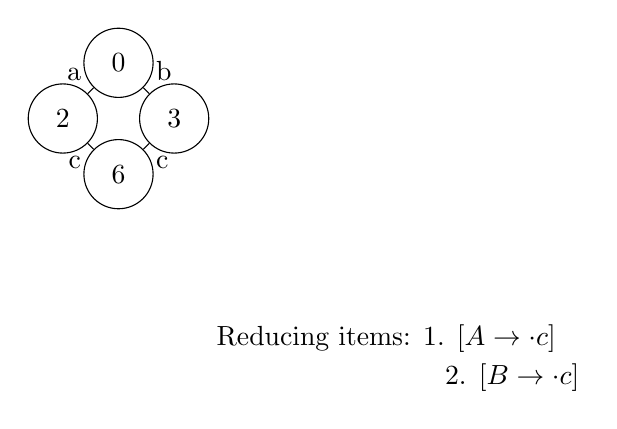
\begin{tikzpicture}
        \node[align=right] at (3.4, -3.5) {Reducing items: 1. $[A \to \cdot c]$};
        \node[align=right] at (5, -4) {2. $[B \to \cdot c]$};
        \node[state] (0) {0};
        \node[state, below left of=0] (2) {2};
        \node[state, below right of=0] (3) {3};
        \node[state, below right of=2] (6) {6};
        \draw (0) edge[above left] node{a} (2)
        (0) edge[above right] node{b} (3)
        (2) edge[below left] node{c} (6)
        (3) edge[below right] node{c} (6)
        ;

    \end{tikzpicture}
\end{document}

